\chapter{Context-aware and recommender systems}
\label{cha:recommenders}

Both topics---context-aware systems and recommender systems---have been growing more and more popular among researchers lately. Both can be discerned to have approximately equivalent curves on accumulated paper and citation counts in time, as shown in \cref{fig:scholar-context-aware} and \cref{fig:scholar-recommender-systems}. Result were obtained after processing 8098 and 3420 papers, respectively, that is all papers that have been found for ``recommender systems'' and ``context-aware'' queries in Google Scholar and Microsoft Academic Search. The S-like shape of the curves might suggest that the topic has already been researched thoroughly.

\begin{figure}
	\centering
	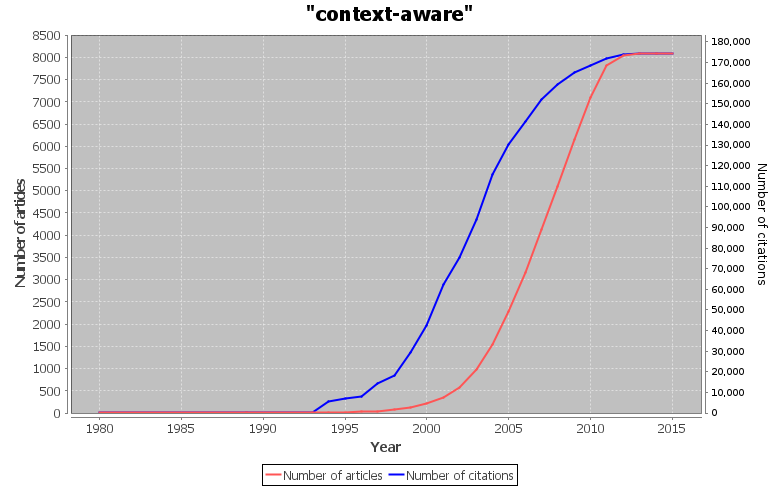
\includegraphics[width=\textwidth]{scholar-context-aware}
	\caption{Google Scholar and Microsoft Academic Search accumulated trending for ``context-aware'' query \cite{Rus:scholar-trends}.}
	\label{fig:scholar-context-aware}
\end{figure}

\begin{figure}
	\centering
	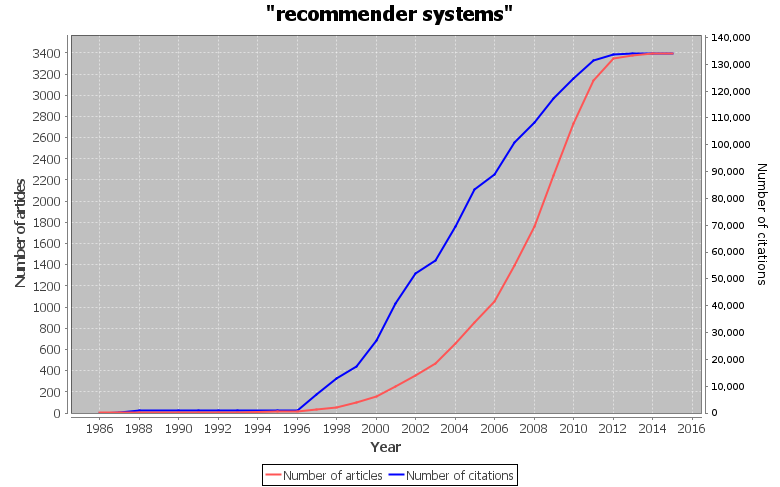
\includegraphics[width=\textwidth]{scholar-recommender-systems}
	\caption{Google Scholar and Microsoft Academic Search accumulated trending for ``recommender systems'' query \cite{Rus:scholar-trends}.}
	\label{fig:scholar-recommender-systems}
\end{figure}

\section{Context-aware systems}
\label{sec:context-aware}

The term, context-awareness, refers to the ability of the system to sense/be aware of its environment. This term mainly applies to mobile systems which are more likely to have their surroundings changed frequently. It is in a way similar to location awareness but expands beyond just location. Various researchers identify different elements of the context, e.g.:

\begin{itemize}
	\item user, role, identity \cite{Dey:context} \cite{Kaltz:context},
	\item process, task \cite{Kaltz:context},
	\item location \cite{Dey:context} \cite{Kaltz:context},
	\item time \cite{Dey:context} \cite{Kaltz:context},
	\item device \cite{Kaltz:context},
	\item activity \cite{Dey:context},
	\item nearby people and devices \cite{Rosslin:context},
	\item lighting and noise level \cite{Rosslin:context},
	\item network availability \cite{Rosslin:context},
	\item even the social situation (relations between the user and their peers nearby) \cite{Rosslin:context}.
\end{itemize}

By keeping track of this variables over the period of time, a system that would be classified as a context-aware one, could infer things that would be useful to the user. These might include turning on appropriate application on a mobile device when a certain set of conditions is met etc.

Context awareness is also an important concept in so called ubiquitous computing or just \emph{ubicomp}. To the regular user, ubicomp---also called pervasive computing and, more recently and commercially, Internet of Things---appears as if the computing processes were happening literally anywhere between a large network of distributed devices. These small, inexpensive devices equipped with various sensors share information among themselves as well as with services run by manufacturers, in order to provide the end user with some greater value.

Some exemplary use cases for a ubiquitous system might include:

\begin{itemize}
	\item ``domestic ubiquitous computing environment might interconnect lighting and environmental controls with personal biometric monitors woven into clothing so that illumination and heating conditions in a room might be modulated, continuously and imperceptibly'' \cite{wiki:ubiquitous},
	\item ``refrigerators «aware» of their suitably tagged contents, able to both plan a variety of menus from the food actually on hand, and warn users of stale or spoiled food'' \cite{wiki:ubiquitous}.
\end{itemize}

Thus, it is safe to say that ubiquitous computing would not be able to function without context-awareness.

An interesting research that is taking place in recent years, and is definitely worth taking a closer look at, concerns data gathered by the AWARE Framework.

AWARE Framework is an application and a library with a main purpose of gathering mobile context information. Analyzed sensors include: accelerometer, barometer, battery, running applications, Bluetooth, communication activities, gravity, gyroscope, locations, the level of light, network connectivity, temperature and many more. \cite{aware}

The collected data is sent to a pre-configured web service running a SQL data base in the back-end, where it can afterwards be analyzed by researchers. Furthermore it provides non-academic developers to enhance User Experience of their applications. By using the context information, they are able to plan notification/interruption moments more sanely. \cite{aware}

Choosing which elements of context are relevant for a given case is quite demanding, as there are many points to take into consideration. As AWARE developers put it, ``Capturing context is challenging. In fact, context is produced anytime, anywhere, by everything and anyone: it is extremely volatile and subjective.'' \cite{aware} One also has to think of such a mundane question as\ldots battery life of the mobile device.

\vspace{4cm}
\todo{cite something by S. Bobek}
\clearpage

\section{Recommender systems}

According to \cite{Ricci:recommenders}, recommender systems are computer systems that may be used to predict ratings their users would give to certain items. In other words, these systems are able to predict (obviously, to some degree of correctness) which items would be most likely to be chosen by the user to interact with. In recent years, the solutions grew in popularity so much, that it is hard to imagine our digital lives without them. Classes of recommended items include:

\begin{itemize}
	\item entertainment: books, music, news, movies,
	\item restaurants, concerts, museums, places in general,
	\item interestingly, search queries (when we get intelligent suggestions after starting to type our queries into Google's search engine),
	\item help with (semi-)manual classification: hash-tags, social tags, question tags on question-oriented sites like Quora or StackExchange etc.,
	\item contacts: new friends on Facebook (the ``Friends \& People You May Know'' feature), new people to follow on Twitter (the ``Who To Follow'' or ``WTF'' feature) and also people one might be interested in on online dating services,
	\item financial services, life insurance policies. \cite{Felfernig:recommenders}
\end{itemize}

Recommender systems can be divided into three types.

\begin{enumerate}
	\item Collaborative filtering.
	\item Content-based filtering.
	\item Any mix of the two above (the so-called \emph{hybrid recommender systems}).
\end{enumerate}

\subsection{Collaborative filtering}

Collaborative filtering method works by looking at user's past behaviors, comparing them to other users of the system, finding most similar users and recommending items based on their decisions in the past. This model has several drawbacks (which, again, depend on the point of view):

\begin{itemize}
	\item a rather large amount of data is required for the system to provide valuable insight (the \emph{cold start} problem),
	\item at the same time care must be taken to make the system scalable; often, these systems face millions and millions of users and items,
	\item sparsity and scarcity of data (user explicit or implicit ratings) --- again, as there are millions of items, it is often the case that only some of the items are rated and theres not enough data to make necessary connections,
	\item all current realizations assume that users agreeing in the past will agree in the future (future understood as the recommendations to be made), which might not always be true.
\end{itemize}

The sparsity problem can be solved by inventing better methods of obtaining user ratings. These ratings can be generally classified 

While explicitness of asking a user to rate a movie is understandable---after all few people would complain, as it is obvious that the movie recommending system has to learn our likes and dislikes to build the proper model of our brains (and going through the movies we watched again and rating them is fun, too!)---when we start getting into e-commerce areas, it stops being justified right away.

This phenomenon might be explained psychologically. When interacting with a movie recommender, the person wants to get some great new recommendations, they are willing to pay for them with their ratings. On the other hand, the commercial recommender is seen as one wanting to take advantage of the user, make them buy some more items and in turn make even more money. This negative image can only be overturned by the system recommending just the right items (from the user's perspective).

One of the most popular collaborative filtering algorithms is the \emph{item--to--item} one, originally popularized by Amazon (the ``people \todo{mention explainability}who buy A buy also B'' feature), used also by Facebook and LinkedIn and Twitter for new friends and groups suggestions, and Last.fm for new music recommendations.

\subsection{Content-based filtering}

The second approach to recommending is content-based filtering. These methods are in turn based on comparing distinctive features of the recommended items to the user's preferences, instead of on what other people (similar to the user) think of them.